\documentclass[11pt,preprint, authoryear]{elsarticle}

\usepackage{lmodern}
%%%% My spacing
\usepackage{setspace}
\setstretch{1.2}
\DeclareMathSizes{12}{14}{10}{10}

% Wrap around which gives all figures included the [H] command, or places it "here". This can be tedious to code in Rmarkdown.
\usepackage{float}
\let\origfigure\figure
\let\endorigfigure\endfigure
\renewenvironment{figure}[1][2] {
    \expandafter\origfigure\expandafter[H]
} {
    \endorigfigure
}

\let\origtable\table
\let\endorigtable\endtable
\renewenvironment{table}[1][2] {
    \expandafter\origtable\expandafter[H]
} {
    \endorigtable
}


\usepackage{ifxetex,ifluatex}
\usepackage{fixltx2e} % provides \textsubscript
\ifnum 0\ifxetex 1\fi\ifluatex 1\fi=0 % if pdftex
  \usepackage[T1]{fontenc}
  \usepackage[utf8]{inputenc}
\else % if luatex or xelatex
  \ifxetex
    \usepackage{mathspec}
    \usepackage{xltxtra,xunicode}
  \else
    \usepackage{fontspec}
  \fi
  \defaultfontfeatures{Mapping=tex-text,Scale=MatchLowercase}
  \newcommand{\euro}{€}
\fi

\usepackage{amssymb, amsmath, amsthm, amsfonts}

\def\bibsection{\section*{References}} %%% Make "References" appear before bibliography


\usepackage[round]{natbib}

\usepackage{longtable}
\usepackage[margin=2.3cm,bottom=2cm,top=2.5cm, includefoot]{geometry}
\usepackage{fancyhdr}
\usepackage[bottom, hang, flushmargin]{footmisc}
\usepackage{graphicx}
\numberwithin{equation}{section}
\numberwithin{figure}{section}
\numberwithin{table}{section}
\setlength{\parindent}{0cm}
\setlength{\parskip}{1.3ex plus 0.5ex minus 0.3ex}
\usepackage{textcomp}
\renewcommand{\headrulewidth}{0.2pt}
\renewcommand{\footrulewidth}{0.3pt}

\usepackage{array}
\newcolumntype{x}[1]{>{\centering\arraybackslash\hspace{0pt}}p{#1}}

%%%%  Remove the "preprint submitted to" part. Don't worry about this either, it just looks better without it:
\makeatletter
\def\ps@pprintTitle{%
  \let\@oddhead\@empty
  \let\@evenhead\@empty
  \let\@oddfoot\@empty
  \let\@evenfoot\@oddfoot
}
\makeatother

 \def\tightlist{} % This allows for subbullets!

\usepackage{hyperref}
\hypersetup{breaklinks=true,
            bookmarks=true,
            colorlinks=true,
            citecolor=blue,
            urlcolor=blue,
            linkcolor=blue,
            pdfborder={0 0 0}}


% The following packages allow huxtable to work:
\usepackage{siunitx}
\usepackage{multirow}
\usepackage{hhline}
\usepackage{calc}
\usepackage{tabularx}
\usepackage{booktabs}
\usepackage{caption}


\newenvironment{columns}[1][]{}{}

\newenvironment{column}[1]{\begin{minipage}{#1}\ignorespaces}{%
\end{minipage}
\ifhmode\unskip\fi
\aftergroup\useignorespacesandallpars}

\def\useignorespacesandallpars#1\ignorespaces\fi{%
#1\fi\ignorespacesandallpars}

\makeatletter
\def\ignorespacesandallpars{%
  \@ifnextchar\par
    {\expandafter\ignorespacesandallpars\@gobble}%
    {}%
}
\makeatother

\newenvironment{CSLReferences}[2]{%
}

\urlstyle{same}  % don't use monospace font for urls
\setlength{\parindent}{0pt}
\setlength{\parskip}{6pt plus 2pt minus 1pt}
\setlength{\emergencystretch}{3em}  % prevent overfull lines
\setcounter{secnumdepth}{5}

%%% Use protect on footnotes to avoid problems with footnotes in titles
\let\rmarkdownfootnote\footnote%
\def\footnote{\protect\rmarkdownfootnote}
\IfFileExists{upquote.sty}{\usepackage{upquote}}{}

%%% Include extra packages specified by user

%%% Hard setting column skips for reports - this ensures greater consistency and control over the length settings in the document.
%% page layout
%% paragraphs
\setlength{\baselineskip}{12pt plus 0pt minus 0pt}
\setlength{\parskip}{12pt plus 0pt minus 0pt}
\setlength{\parindent}{0pt plus 0pt minus 0pt}
%% floats
\setlength{\floatsep}{12pt plus 0 pt minus 0pt}
\setlength{\textfloatsep}{20pt plus 0pt minus 0pt}
\setlength{\intextsep}{14pt plus 0pt minus 0pt}
\setlength{\dbltextfloatsep}{20pt plus 0pt minus 0pt}
\setlength{\dblfloatsep}{14pt plus 0pt minus 0pt}
%% maths
\setlength{\abovedisplayskip}{12pt plus 0pt minus 0pt}
\setlength{\belowdisplayskip}{12pt plus 0pt minus 0pt}
%% lists
\setlength{\topsep}{10pt plus 0pt minus 0pt}
\setlength{\partopsep}{3pt plus 0pt minus 0pt}
\setlength{\itemsep}{5pt plus 0pt minus 0pt}
\setlength{\labelsep}{8mm plus 0mm minus 0mm}
\setlength{\parsep}{\the\parskip}
\setlength{\listparindent}{\the\parindent}
%% verbatim
\setlength{\fboxsep}{5pt plus 0pt minus 0pt}



\begin{document}



\begin{frontmatter}  %

\title{Question 3: Portfolio construction and comparison}

% Set to FALSE if wanting to remove title (for submission)




\author[Add1]{Austin Byrne}
\ead{22582053@sun.ac.za}





\address[Add1]{Stellenbosch University, Stellenbosch, South Africa}

\cortext[cor]{Corresponding author: Austin Byrne}

\begin{abstract}
\small{
The purpose of this question is to construct a portfolio analysis on the
weighted ALSI and weighted SWIX portfolios. In this question I will plot
the cumulative returns of both portfolios and evaluate the comparisons
and differences. Furthermore, a breakdown of the various weighted
contributions of each sector within each weighted portfolio will be
analysed.
}
\end{abstract}

\vspace{1cm}





\vspace{0.5cm}

\end{frontmatter}

\setcounter{footnote}{0}



%________________________
% Header and Footers
%%%%%%%%%%%%%%%%%%%%%%%%%%%%%%%%%
\pagestyle{fancy}
\chead{}
\rhead{}
\lfoot{}
\rfoot{\footnotesize Page \thepage}
\lhead{}
%\rfoot{\footnotesize Page \thepage } % "e.g. Page 2"
\cfoot{}

%\setlength\headheight{30pt}
%%%%%%%%%%%%%%%%%%%%%%%%%%%%%%%%%
%________________________

\headsep 35pt % So that header does not go over title




\hypertarget{introduction}{%
\section{\texorpdfstring{Introduction
\label{Introduction}}{Introduction }}\label{introduction}}

Using the information on the ALSI (J203) and SWIX (J403) Indexes, I will
be writing a short report where I will be comparing the specific
methodologies used by the ALSI and the SWIX, evaluating the cumulative
returns of each and plotting them together to perform a comparison,
evaluating which sectors hold the highest weight and contribution for
each.

\hypertarget{loading-relevant-data-and-packages}{%
\section{Loading relevant data and
packages}\label{loading-relevant-data-and-packages}}

The data used is data based on the ALSI and SWIX. The data contains
dates, weights and returns for each.

\hypertarget{lets-create-an-alsi-and-swix-weighted-poerfolio-cumulative-returns}{%
\section{Lets create an ALSI and SWIX weighted poerfolio cumulative
returns}\label{lets-create-an-alsi-and-swix-weighted-poerfolio-cumulative-returns}}

\hypertarget{first-lets-calculate-each-indexes-weighted-daily-portfolio-returns-using-the-safe_returns}{%
\subsection{First lets calculate each indexes weighted daily portfolio
returns using the
safe\_returns:}\label{first-lets-calculate-each-indexes-weighted-daily-portfolio-returns-using-the-safe_returns}}

In order to use the safe\_returns function to calculate the weighted
portfolio returns I need to convert the data to and xts format. That is
done below:

Now that we have the merged data frame of portfolio returns for the ALSI
and SWIX in the correct format, I can move onto calculating the
cumulative weighted returns.

\hypertarget{cumulative-returns-plot}{%
\subsection{Cumulative returns plot}\label{cumulative-returns-plot}}

\begin{figure}[H]

{\centering 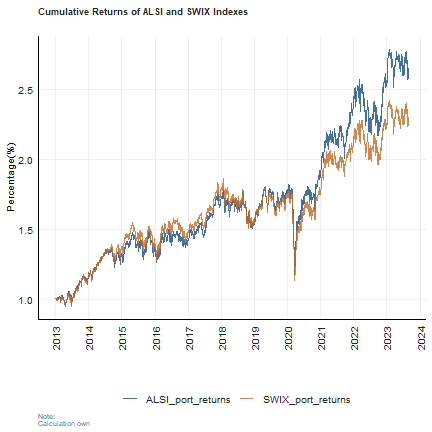
\includegraphics{Question-3_files/figure-latex/Figure 1-1} 

}

\caption{Cumulative returns plot \label{Figure1}}\label{fig:Figure 1}
\end{figure}

As can be seen from the above graph, the cumulative returns for the ALSI
and the SWIX were very similar until 2020, at which point the ALSI began
outperforming the SWIX. Immediate prior to this separation in cumulative
returns was a huge draw down for both the ALSI and SWIX weighted
portfolios. Since this draw down is within 2020, a possible reason could
be the COVID-19 pandemic. There may have been a switch in weights
between the two portfolios which would result in varying returns. From
the graph it is evident that the ALSI reacted better than the SWIX to
this heavy draw down in 2020.

To further this analysis I will dive into the weighted construction of
the ALSI and SWIX portfolios, more precisely, I will be analyzing the
weighted return contribution for each sector and evaluating the
differences in the ALSI and SWIX.

\hypertarget{each-sectors-weighted-return-contribution}{%
\subsection{Each sectors weighted return
contribution}\label{each-sectors-weighted-return-contribution}}

In this section of code I am grouping by sector to then be able to
calculate the weighted reuturn contribution of each sector in the
respective ALSI and SWIX portfolios. I can then evaluate which sectors
are the main drivers to portfolio returns.

\hypertarget{the-alsis-individual-sectors-weighted-return-contribution}{%
\subsection{The ALSI's individual sectors weighted return
contribution}\label{the-alsis-individual-sectors-weighted-return-contribution}}

Here we are able to evaluate which sector(s) are the main weighted
return drivers of the ALSI weighted portfolio. From the plot below it is
evident that for the last 10 years the majority of the return in the
ALSI weighted portfolio has come from the Industrial sector and the
lowest coming from the property/residual sectors. However, since 2016
the industrial sector has slowly started lossing its majority hold to an
ever rising contribution from the resources sector.

Next we are going to evaluate the same plot but for the SWIX weighted
portfolio. We will then be able to do identify a possibility of why the
cumulative returns of the two portfolios differ.

\begin{figure}[H]

{\centering 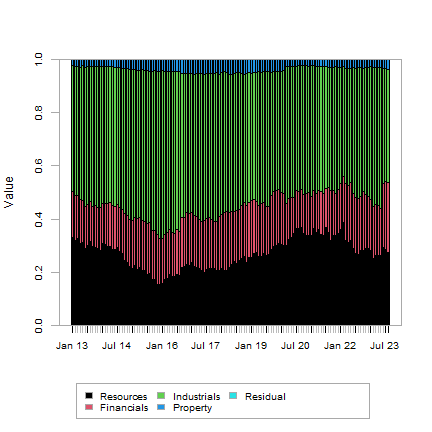
\includegraphics{Question-3_files/figure-latex/Figure 2-1} 

}

\caption{ALSI sector contribution plot \label{Figure2}}\label{fig:Figure 2}
\end{figure}

\hypertarget{the-swixs-individual-sectors-weighted-return-contribution}{%
\subsection{The SWIX's individual sectors weighted return
contribution}\label{the-swixs-individual-sectors-weighted-return-contribution}}

The plot below evaluates which sector(s) are the main weighted return
drivers of the SWIX weighted portfolio. Like that of the ALSI, the
majority holding is found in the industrial sector with again the
minority held by the the property/residual sectors. The trajectory of
increased contribution from the resources sector is scene here again as
was seen in the ALSI portfolio. However, the differences lie in the
actual value. It is evident that the SWIX weighted portfolio has a more
even contribution between the financial sector and resources sector.
Where the ALSI has a higher contribution from the resources sector over
the financial sector.

\begin{figure}[H]

{\centering 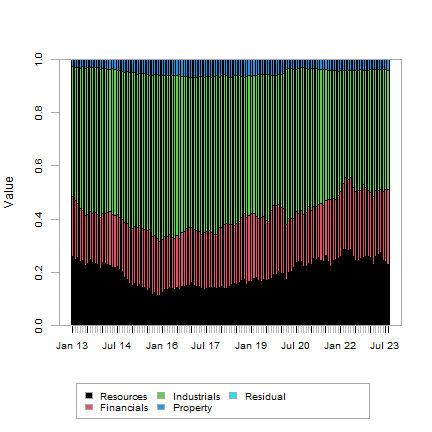
\includegraphics{Question-3_files/figure-latex/Figure 3-1} 

}

\caption{SWIX sector contribution plot \label{Figure3}}\label{fig:Figure 3}
\end{figure}

\hypertarget{comparisson-of-the-alsi-and-swix-portfolio-contribution}{%
\subsection{Comparisson of the ALSI and SWIX portfolio
contribution}\label{comparisson-of-the-alsi-and-swix-portfolio-contribution}}

When evaluating the weighted contributions of the various sectors to the
ALSI and SWIX portfolios, there are some similarities but also some
points of difference. Both portfolios have a large contribution from the
industrial sector. Where the differences play a part is with respect to
the financial a resources sectors. The ALSI obtains more weight from the
resource sectors over that of the financial sector, while the SWIX
obtains more of an even split between the two. This difference may be
the contributing factor as to why the ALSI performed better than the
SWIX since 2020.

\newpage

\hypertarget{references}{%
\section*{References}\label{references}}
\addcontentsline{toc}{section}{References}

\hypertarget{refs}{}
\begin{CSLReferences}{0}{0}
\end{CSLReferences}

\hypertarget{appendix}{%
\section*{Appendix}\label{appendix}}
\addcontentsline{toc}{section}{Appendix}

\hypertarget{appendix-a}{%
\subsection*{Appendix A}\label{appendix-a}}
\addcontentsline{toc}{subsection}{Appendix A}

Some appendix information here

\hypertarget{appendix-b}{%
\subsection*{Appendix B}\label{appendix-b}}
\addcontentsline{toc}{subsection}{Appendix B}

\bibliography{Tex/ref}





\end{document}
